\documentclass[11pt]{report}


%%%%%%%%%%%%%%%%%%%%%%%%%%%%%%
%Import Packages

\usepackage{graphicx}
\usepackage{titlesec}
\usepackage{caption}
\usepackage[table]{xcolor}
%%%%%%%%%%%%%%%%%%%%%%%%%%%%%%


%%%%%%%%%%%%%%%%%%%%%%%%%%%%%%
% Other commands

\titleformat{\chapter}{\normalfont\huge}{}{20pt}{\huge\bf}
%%%%%%%%%%%%%%%%%%%%%%%%%%%%%%


\begin{document}


%%%%%%%%%%%%
%Template for Figures %
%%%%%%%%%%%%

\begin{figure}[ht!]
\centering

\includegraphics[width=90mm]{./Sprint2/img/Sprint2-GitnGithub.png}
\caption{Git and GitHub \label{overflow}}
\end{figure}


%%%%%%%%%%%%%
%Template for sideways figures %
%%%%%%%%%%%%%

\afterpage{
\clearpage
\begin{landscape}
    \centering
    \begin{figure}
        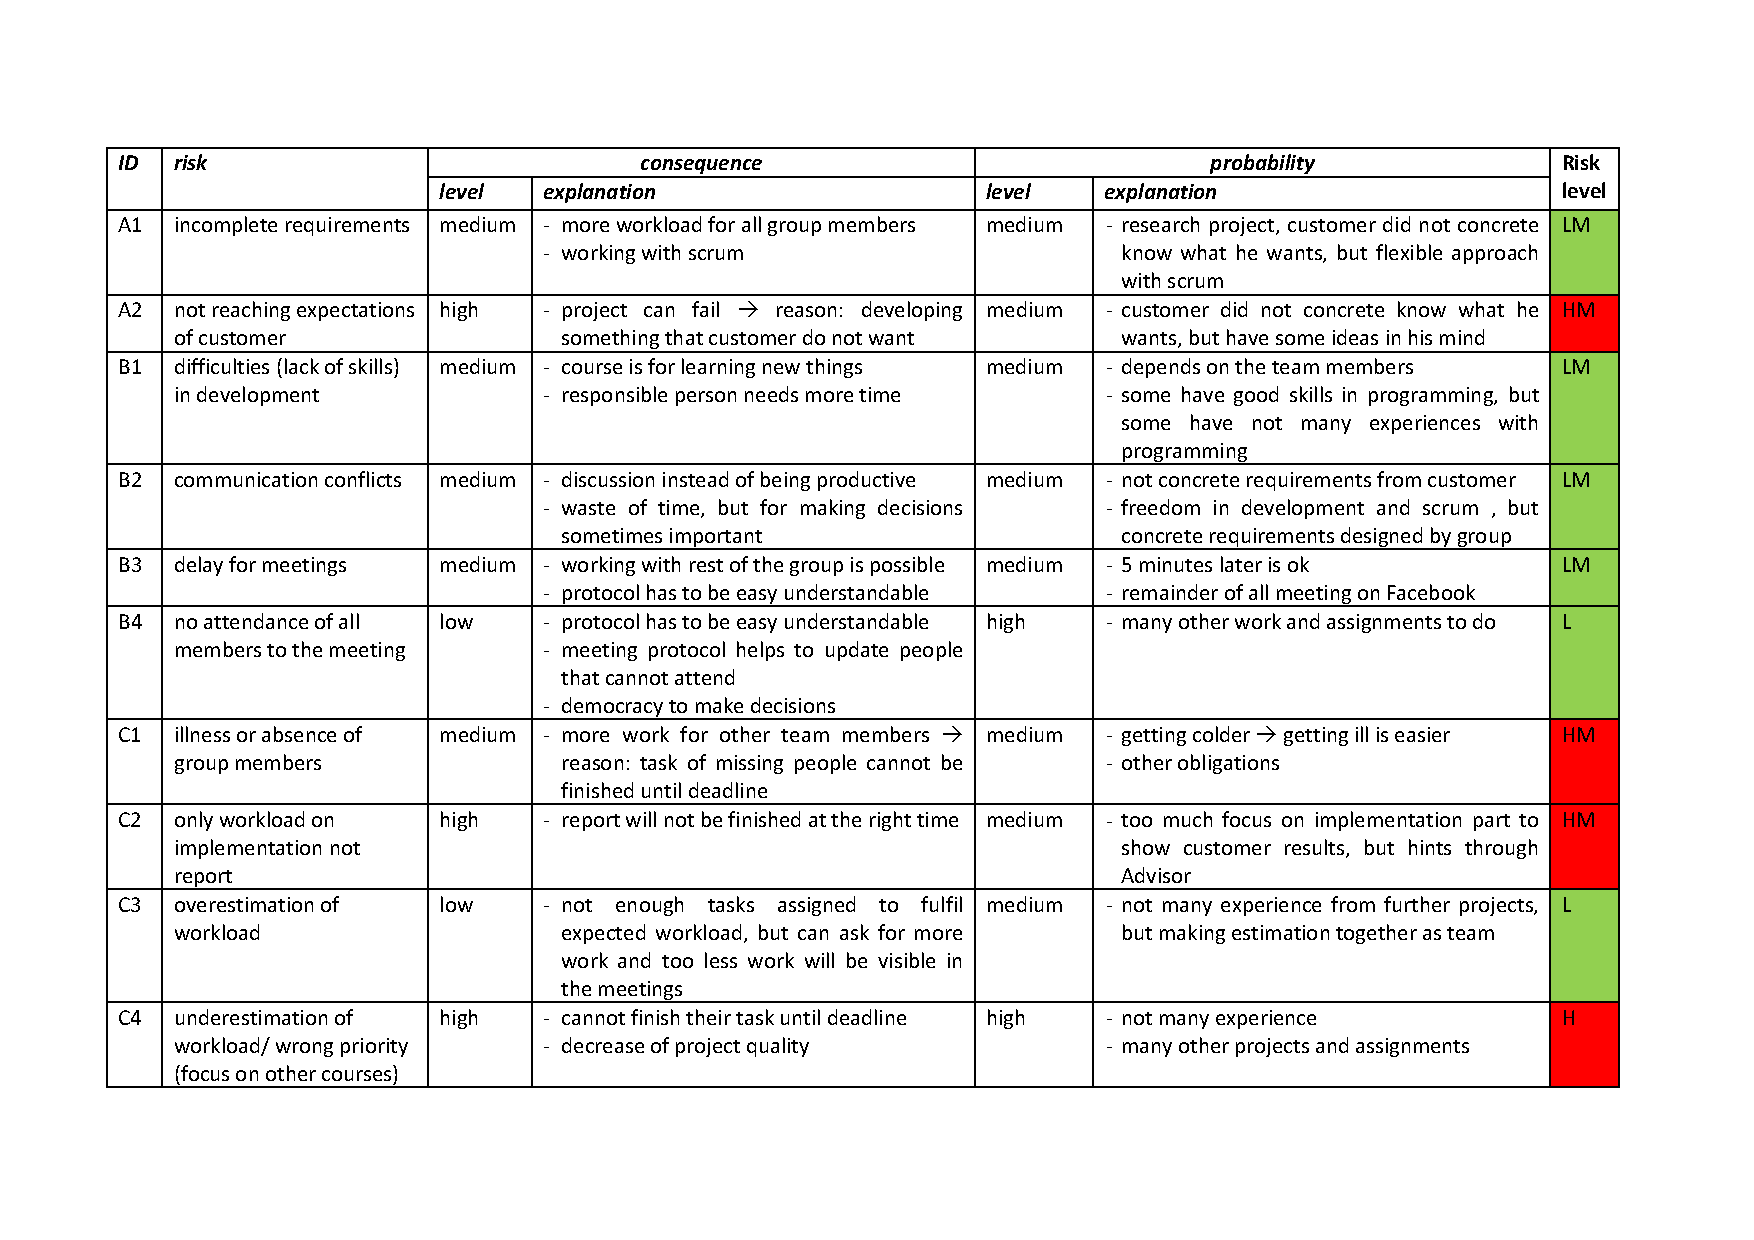
\includegraphics[width=\linewidth]{./Introduction/img/Risk.pdf}
        \caption{Risks for the Alternative Spaces project.}
        \label{fig:IntroRiskManRisks}
    \end{figure}
\end{landscape}
}


%%%%%%%%%%%%%%%%
%Template for Sprint Duration %
%%%%%%%%%%%%%%%%

\begin{minipage}{\linewidth}
\centering
\setlength{\tabcolsep}{22pt}
\textbf{Sprint 2:} 
\smallskip
\rowcolors{1}{blue!20}{blue!10}
\begin{tabular}{ |l l| }
	\hline
	\it{Duration} & 1 week \\
	\it{Start} & September 22nd. \\
	\it{End} & September 28th. \\
	\it{Workload} & Hours spent by the entire group on Sprint 2. \\
	\it{Goal} & 20-25 hours per person \\
	\hline
\end{tabular}
\end{minipage}



%%%%%%%%%%%%%%%%
%Template for workload table  %
%%%%%%%%%%%%%%%%

\begin{minipage}{\linewidth}
\setlength{\tabcolsep}{15pt}
\centering
\rowcolors{1}{blue!20}{blue!10}
\begin{tabular}{ |l|l| }
	\hline
	\multicolumn{2}{|c|}{\cellcolor{gray!25} Workload} \\
	\hline
	\it{Work item 1} & X hrs\\
	\it{Work item 2} & Y hrs\\
	\it{Work item 3} & Z hrs\\
	\hline
	\textbf{\textit{Total Workload}} & A hrs\\
	\hline
\end{tabular}
%Caption here
\captionof{table}{Workload of Sprint X.} 
\end{minipage}



%%%%%%%%%%%%%%%%%%%
%Template for Sprint Backlog table    %
%%%%%%%%%%%%%%%%%%%
\begin{minipage}{\linewidth}
\setlength{\tabcolsep}{12pt}
\centering
\rowcolors{1}{blue!20}{blue!10}
\begin{tabular}{|p{1cm}|p{4cm}|p{2cm}|p{2cm}|}
\hline
\cellcolor{gray!25} ID & \cellcolor{gray!25} Description & \cellcolor{gray!25} Estimated Time & \cellcolor{gray!25} Actual Time \\
\hline
TA2.1 & \it{Structurize google drive folders, and use the same language in all documents.} & 1 week & 15 hours \\
TA2.2 & \it{Set up NTNU home area for running and testing code.} & 1 hour & 1 hour \\
TE2.3 & \it{Use NTNU-s MySQL server over SSH for testing database of user sign up, user creation, validation etc. } & 1 week & 4 hours \\
D2.4.1 & \it{Find and apply a theme color for the webpage. } & 1 week & 15 hours \\
\hline
\end{tabular}
\captionof{table}{Backlog for sprint 1.} 
\end{minipage}

%%%%%%%%%%%%%%%%%%%%%%%%%%%
% Use case table template %
%%%%%%%%%%%%%%%%%%%%%%%%%%%

\begin{minipage}{\linewidth}
\rowcolors{1}{blue!20}{blue!10}
\begin{tabular}{|l|p{7cm}|}
  \hline
  \multicolumn{2}{|c|}{\cellcolor{gray!25} \textbf{Use case name}} \\
  \hline
  Brief Description & \\
  Preconditions & \\
  Flow &
    \begin{enumerate}
      \item ........
    \end{enumerate} \\
  Basic flow & \\
  Alternative Flows & 
    \begin{itemize}
      \item .........
    \end{itemize} \\
  Special Requirements & \\
  Postconditions & \\
  Extension Points & \\
  \hline
\end{tabular}
\captionof{table}{Use case for X. \label{tab:label}}
\end{minipage}

%%%%%%%%%%%%%%%%%%%%%%%%%%%%%%%%%%%
% Template for code documentation %
%%%%%%%%%%%%%%%%%%%%%%%%%%%%%%%%%%%
\subsubsection{DBComments}
\begin{minipage}{\linewidth}
  \centering
  \setlength{\tabcolsep}{12pt}
  \rowcolors{1}{blue!20}{blue!10}
  \begin{tabular}{|p{0.35\linewidth}|p{0.55\linewidth}|}
  \hline
  \cellcolor{gray!25} Function & \cellcolor{gray!25} Description \\
  \hline
  getComments(threadID) & Fetching all comments related to a threadID from the database. \\
  insertComment(threadID, parent, username, comment) & Inserts a new comment into the database. All comments have a creator (username), a threadID and the comment itself. If the comment is a reply, it also has a parent comment. \\
  \hline  
  \end{tabular}
\end{minipage}


%%%%%%%%%%%%%%%%%%%%%%%%%%
% Templates for labeling %
%%%%%%%%%%%%%%%%%%%%%%%%%%

\chapter{Introduction}
\label{chap:Intro}

\section{Description}
\label{sec:IntroDescr}

\subsection{Name}
\label{subsec:IntroDescrName}

%Figure:
\label{fig:FigName}

%Table:
\label{tab:TabName}

%To reference:
See chapter \ref{chap:Intro}

\end{document}